\documentclass[a4paper,10pt]{scrartcl}
\usepackage[utf8]{inputenc}
\usepackage[spanish]{babel} 
\usepackage[hidelinks]{hyperref}
\usepackage{color}
\usepackage{graphicx}
\usepackage{enumitem}
\usepackage{float}
\graphicspath{ {images/} }


\title{Ejercicio práctico Redmine}
\subtitle{Grupo 1.2.2 - Redmine}
\author{
		Manuel Francisco López Ruiz\\
		Julio Márquez Castro\\
		Álvaro Martín Gordillo\\
		  }

\begin{document}

\clearpage\maketitle
\thispagestyle{empty}
\newpage

\newpage

\tableofcontents

\newpage

\section{Contexto}

Una empresa de desarrollo de aplicaciones móviles decide usar la herramienta Redmine para controlar un proyecto ya iniciado encargado por un cliente. Una aplicación nativa Android. Su objetivo principal es el control remoto de un dron mediante cualquier dispositivo con Android.\\

El proyecto comenzó el 5/09/2016 y actualmente se encuentra en la fase de Producción, concretamente en la Implementación. Están teniendo dificultades en esta fase, esto puede ocasionarles un retraso en la fase actual y el jefe de proyecto ha decidido asignarle una prioridad superior.\\

El jefe del proyecto ha decidido crear un foro llamado “Variaciones del proyecto”, con descripción “Comunicación para que queden registradas posibles variaciones en el proyecto” y un mensaje de bienvenida: “Cualquier idea que pueda mejorar el proyecto debe ser expuesta en este foro, con idea de que todos los integrantes del equipo de trabajo estén al corriente y pueden comentar sobres estas nuevas ideas”.\\

Las tareas del proyecto no pueden empezar sin acabar la anterior, excepto las de diseño y arquitectura que se realizan al mismo tiempo.\\

El proyecto tiene como fecha límite para desplegar la aplicación el 01/04/2017. 


\section{Equipo de trabajo}


\begin{itemize}{}{}
	\item \textbf{Analista:} responsable de entender las necesidades del cliente, y asegurarse de que la solución que está siendo desarrollada se ajusta a esas necesidades.
	\item \textbf{Jefe del proyecto:} responsable de la planificación del proyecto, de mantener el proyecto dentro del presupuesto, y de la solución de problemas.
	\item \textbf{Arquitecto del Sistema:} responsable de pensar el sistema antes de construirlo. Responsable del software y del hardware.
	\item \textbf{Desarrollador de Software:} implementa las ideas del arquitecto, y como tal, puede tener que discutir las (in)posibilidades de la implementación con el arquitecto.
\end{itemize}

\newpage

\section{Fases del proyecto}


\begin{enumerate}
	\item \textbf{Diseño y arquitectura:} clarificar los objetivos del proyecto, plantear la estrategia más adecuada para el desarrollo del mismo, así como describir la funcionalidad a implementar definiendo su alcance
	\begin{enumerate}[label*=\arabic*.]
		\item \textbf{Análisis funcional y tecnológico:} Definición de los objetivos a alcanzar, y 	descripción modular detallada de los requerimientos del proyecto.
		\item \textbf{Maqueta:} Definición de la línea gráfica de interfaz.
		\item \textbf{Planificación:} Plan detallado del proyecto, asignación de recursos y definición de entregables.
	\end{enumerate}
	
	\item \textbf{Producción:} Consiste en el desarrollo del proyecto organizado en hitos y entregables y así facilitar a los clientes la posibilidad de revisar la aplicación a medida que se va construyendo.
	\begin{enumerate}[label*=\arabic*.]
		\item \textbf{Prototipo}
		\item \textbf{Diseño de Interfaz} 
		\item \textbf{Creación de base de datos}
		\item \textbf{Implementación} 
		\item \textbf{Pruebas}
	\end{enumerate}
	
	\item \textbf{Control de calidad:} Una vez la aplicación ha sido desarrollada y testada con éxito, pasará por una etapa final de control de calidad previa a la aceptación del cliente.
	\begin{enumerate}[label*=\arabic*.]
		\item \textbf{Reunión final con el cliente}
		\item \textbf{Revisión de la reunión con el cliente}
	\end{enumerate}
	
	\item \textbf{Puesta en marcha:} Finalizado el control de calidad y con la aceptación del cliente, se lleva a cabo la fase de despliegue y puesta en marcha.
	\begin{enumerate}[label*=\arabic*.]
		\item \textbf{Despliegue de la app}
		\item \textbf{Fase de cierre, inicio de la mejora continua y soporte:} Se da por finalizado el proyecto al haberse alcanzado los objetivos consensuados con el cliente, y entra en vigor la garantía. Durante este periodo se pueden analizar ampliaciones funcionales que aporten más valor añadido al proyecto, o nuevas oportunidades de negocio que desemboquen en futuras colaboraciones. Al finalizar la garantía, entrará en vigor el periodo de soporte y mejora continua.
	\end{enumerate}
\end{enumerate}

\newpage

\section{Planificación de tareas}

\begin{center}
	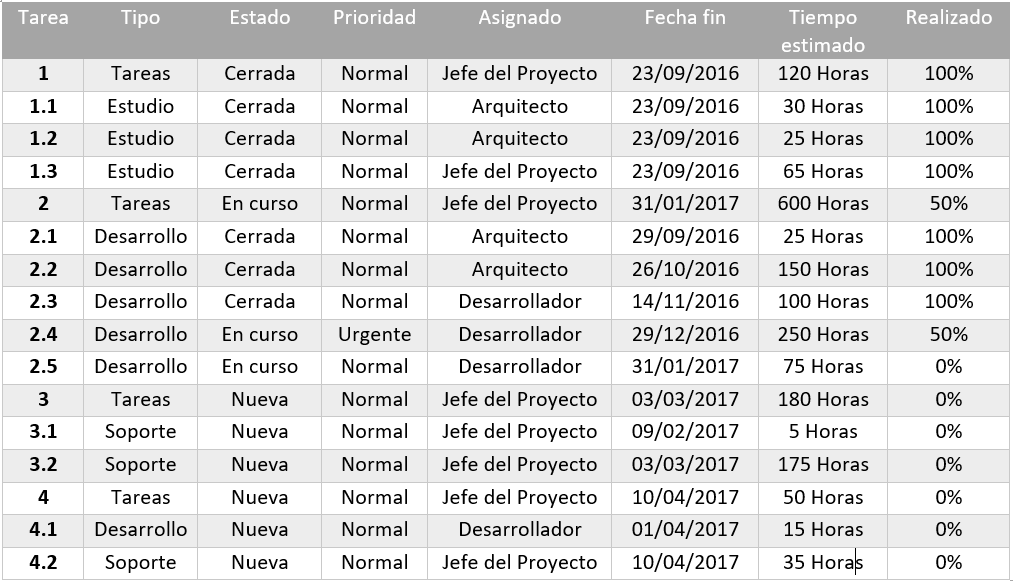
\includegraphics[width=16cm]{tabla}
\end{center}



\bibliography{sample}

\end{document}
